\documentclass{article}

% \usepackage[spanish]{babel}

\usepackage[utf8]{inputenc}

\usepackage{graphicx}

\title{Ecuaciones en diferencias}

\author{Luis Angel Topete Galván}

\date{25 de septiembre de 2017}

\begin{document}

\maketitle

\section{Ecuaciones de primer grado}

\subsection{Ecuaciones lineales}

Una ecuación en diferencias de primer grado tiene la forma $x_{n+1}=ax_n$ donde $a$ es una constante.
La fórmula para resolver ecuaciones lineales es:

\begin{equation}
  \label{eq:lineal}
  x_n=a^nx_0 
\end{equation}

Por ejemplo, si iniciamos una inversión de 1000 pesos con un interes mensual del 1 \% obtenemos lo siguiente :

\begin{center}
  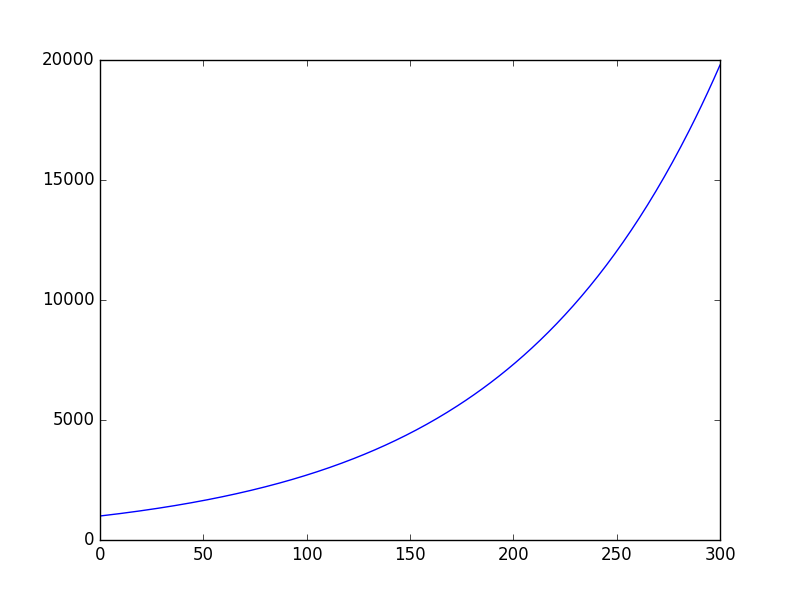
\includegraphics[width=7cm]{Inversion.png}
\end{center}


Una ecuación afín en diferencias de primer grado tiene la forma $x_{n+1}=ax_n+b$ donde $a$ es una constante.
\begin{equation}
 \label{eq:afin}
 x_n=a^n(x_0-\alpha)+\alpha
\end{equation}

Donde $\alpha=\frac{b}{1-a}$.
Para deducir esta fórmula usamos que $$\sum_{i=0}^{n-1}a^i=\frac{a^n-1}{a-1}$$.
\section{Ecuaciones de segundo grado}
\end{document}



